\label{sec:background}
\subsection{CNN based methods in DSLAM}
As described before, there are two essential components on each agent: $1)$ Visual Odometry (VO) and $2)$ Place Recognition.

\subsubsection{Visual Odometry (VO)}

Visual odometry estimation is the task to infer ego-motion from a sequence of images and is an essential component in the SLAM system. Some feature-based SLAM systems have enjoyed great success, like ORB-SLAM\cite{DBLP:journals/trob/Mur-ArtalMT15} and ORB-SLAM2\cite{Mur-Artal:2017281}. Recently, several studies have shown that these feature-based SLAM systems require high computing resources. Fang et al.\cite{Fang2017FPGAbasedOF} shows that the feature extraction stage is the most computation-intensive, consuming over 50\% of the CPU resources.

As FPGA is one of the most promising platforms as the accelerator for VO, the SLAM system on FPGA has become a hot research topic. However, FPGA-accelerated feature extraction still consumes a lot of time and computing resources, which cannot be deployed simultaneously with an FPGA-accelerated neural network.

\subsubsection{Place Recognition}

The goal of place recognition is to calculate a given frame into a limited set of places. Each place can be encoded as a concise code which can be easy transferred with low communication cost. Traditional place recognition method usually translate the input frame as the aggregation of handcrafted feature point and local descriptors, like SIFT \cite{Lowe:2004e6e} or ORB \cite{Mur-Artal:2017281}, using vectorization techniques like bag-of-words (BoW) \cite{Galvez-Lopez:2012c94} or vector of locally aggregated descriptors(VLAD) \cite{Jegou:2010f45}.

Recent advances in the deep learning and the convolution neural network (CNN) enable powerful end-to-end mode for place recognition \cite{Noh:2017d0b, Arandjelovic:2017997}, and the NetVLAD method is one of the most accurate methods based on CNN. The NetVLAD algorithm based on VGG-16 model \cite{Simonyan:20143be} consumes more than $80G$ operations for a single $300 \times 300$ input image (each operation means addition or  multiplication). It is very challenging to deploy the NetVLAD on a traditional embedded hardware platform.

\subsection{Hardware architecture of Zync MPSoC}
The Xilinx Zync MPSoC is a chip with ARM cores and FPGA fabric. The system is illustrated in \cref{fig:plps}. The ARM cores with an embedded Linux operation system are called Processing System (PS). The FPGA fabric is called Programmable Logic (PL). The peripherals like camera and communication unit (WiFi or others) are accessible with PS. The high-bandwidth on-chip AXI interface is used to communicate between PS and PL. PS and PL can also share the DDR to transfer a large volume of data such as each frame of the camera.
Deephi CNN accelerator, which is called DPU \cite{Tech:2019360}, is one of the state-of-the-art accelerators and is famous for high energy efficiency on various CNN structure. We deploy the accelerator on the PL side of Zynq SoC with the help of DPU.

\begin{figure}[t]  
    \centering  
    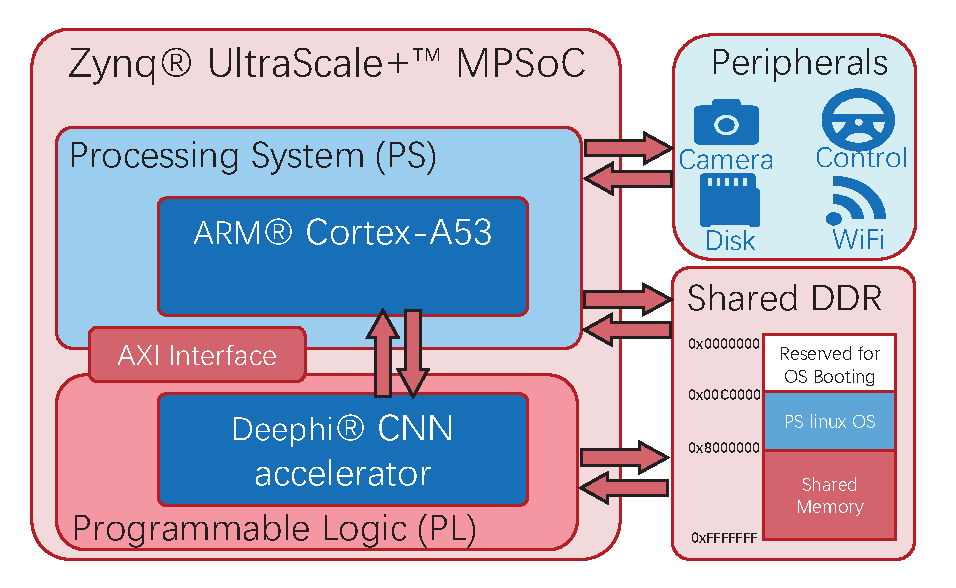
\includegraphics[width=0.95\linewidth]{fig/plps.eps}
    \caption{Hardware architecture of Zynq SoC}
    \label{fig:plps}
\end{figure}

Though FPGA can significantly improve the performance and energy efficiency of CNN inference, FPGA cannot efficiently calculate the floating-point number and requires fixed-point parameters and intermediate data in CNN.

% \subsection{Motivation}
% Though previous work \cite{Cieslewski:20187ee} proposes data-efficient DSLAM system, it is difficult to implement the two essential components, VO and place recognition simultaneously on a communication-limited and energy-constrained embedded hardware platform on a real robot. We propose this hardware-software co-design DSLAM system to use Xilinx Zynq MPSoC and Deephi DPU to execute these two components on the real system.

